\documentclass[french]{report}
\usepackage[utf8]{inputenc}
\usepackage[T1]{fontenc}
\usepackage{lmodern}
\usepackage[a4paper]{geometry}
\usepackage{babel}

%% Pour les images
\usepackage{graphicx}
\usepackage{float}
\usepackage{subfigure} %permet un meilleur affichage d'une image par rapport à une autre
\usepackage{xcolor} %permet d'éviter les conflicts de paquet entre color et xcolor
\renewcommand\thesubfigure{} %pour retirer la numérotation des caption sur les sous figures
\renewcommand\thesubtable{}

%% contrôler mes hauts de page !
\usepackage{fancyhdr} %\usepackage{fancyheadings}

%pour personnaliser les listes
\usepackage{enumerate}

%% pour les url
\usepackage{hyperref} % exemple d'utilisation: \href{www.google.com}{toto}

%% pour les inclusions de fichiers pdf
\usepackage[final]{pdfpages} 

%% Pour les couleurs
%\usepackage{colortbl} %dans les tableaux

%% Définition des newcommand
%% %%%%%%%%%%%%%%%%%%%%%%%%%%%% %
%% INFORMATIONS SUR LE DOCUMENT
%% ---------------------------- %
%% But: Ce fichier contient les 
%% différents accronymes, macro 
%% ...
%% %%%%%%%%%%%%%%%%%%%%%%%%%%%% %


%%%%%%%%%%%%%%%%%%%%%%%%%%%%%%%%%%%%%%%%%%%%%%%%%%%%%%%%%% Les principaux acteurs du projet
\newcommand{\etudiantJP}{Jonathan Poncy}
\newcommand{\etudiantRD}{Romain Daquin}
\newcommand{\etudiantSL}{Stéphane Legrand}
\newcommand{\civiliteResponsableProet}{Monsieur}
\newcommand{\responsableProjet}{Éric Ramat}
\newcommand{\responsableDesProjets}{Julien Dehos}
\newcommand{\pepit}{\href{pepit.be}{Pepit}}
\newcommand{\pepitSite}{\href{http://pepit.be}{pepit.be}}
\newcommand{\pepitMobil}{Pépit Mobil}

%%%%%%%%%%%%%%%%%%%%%%%%%%%%%%%%%%%%%%%%%%%%%%%%%%%%%%%%%% macros techniques
\newcommand{\android}{\href{http://fr.wikipedia.org/wiki/Android}{\textbf{A}ndroid}}
\newcommand{\market}{\gp}
\newcommand{\gp}{\href{http://fr.wikipedia.org/wiki/Google_Play}{Google Play}}
\newcommand{\google}{Google}
\newcommand{\googleDrive}{\google{} Drive}
\newcommand{\os}{\href{http://fr.wikipedia.org/wiki/Syst\%C3\%A8me_d'exploitation}{Système d'Exploitation}}
\newcommand{\eclipse}{\href{http://fr.wikipedia.org/wiki/Eclipse_(logiciel)}{eclipse}}
\newcommand{\ide}{\href{http://fr.wikipedia.org/wiki/Environnement_de_d\%C3\%A9veloppement_int\%C3\%A9gr\%C3\%A9}{I.D.E.}}
\newcommand{\linux}{\href{http://fr.wikipedia.org/wiki/Linux}{Linux}}
\newcommand{\java}{\href{http://fr.wikipedia.org/wiki/Java_(langage)}{Java}}
\newcommand{\github}{\href{http://fr.wikipedia.org/wiki/GitHub}{github}}
\newcommand{\ubuntu}{ubuntu}
\newcommand{\plugin}{plugin}
\newcommand{\plugins}{plugins}

%%%%%%%%%%%%%%%%%%%%%%%%%%%%%%%%%%%%%%%%%%%%%%%%%%%%%%%%%% termes Agiles
\newcommand{\sprint}{\href{http://fr.wikipedia.org/wiki/Scrum\_(m\%C3\%A9thode)\#Le_Sprint}{Sprint}}
\newcommand{\agile}{Agile}%oui, avec un 'A'
\newcommand{\scrum}{\href{http://fr.wikipedia.org/wiki/Scrum\_(m\%C3\%A9thode)}{Scrum}}

%%%%%%%%%%%%%%%%%%%%%%%%%%%%%%%%%%%%%%%%%%%%%%%%%%%%%%%%%% liens
\newcommand{\dossierpdf}{documents_externes/}
\newcommand{\dossierimages}{images/}
%\newcommand{\}{}



%% style des titres
\usepackage{sectsty}
%\convertcolorspec{HTML}{eda299}{RGB}{\toto} pour recuperer un code RGB
%\definecolor{color_chapter}{RGB}{0,0,128}
%\definecolor{color_section}{RGB}{112,147,219}
%\definecolor{color_subsection}{RGB}{19,81,204}
%\chapterfont{\color{color_chapter}{}\fontseries{b}}
%\sectionfont{\color{blue}{}\fontseries{b}}
%\subsectionfont{\color{color_subsection}{}\fontseries{b}}
%\subsubsectionfont{\color{cyan}{}\fontseries{b}}


%% %%%%%%%%%%%%%%%%%%%%%%%%%%%% %
%% INFORMATIONS SUR LE DOCUMENT
%% ---------------------------- %
%% ??? indique un texte à changer
%%
%% tâches (spéciales) à réaliser:
%%  l'ensemble des tâches seront
%%  désormés décrites sur github
%%  sous forme "d'issues"
%%
%% %%%%%%%%%%%%%%%%%%%%%%%%%%%% %
\begin{document}
%% page de titre

\begin{titlepage}

\begin{center}


%% partie supérieur de la page

\includegraphics[width=16cm]{images/pepit-logo}\\[1cm]    

\textsc{\LARGE \textbf{U}niversité du \textbf{L}ittoral \textbf{C}ôte d'\textbf{O}pale}\\[1.5cm]
\textsc{\Large 2\ieme{} année de master informatique}\\[0.5cm]


% Titre
%\HRule \\[0.4cm]
{ \huge \bfseries Rapport de projet}\\[0.4cm]

%\HRule \\[1.5cm]

% Auteurs et superviseurs
\begin{minipage}{0.3\textwidth}
\begin{flushleft} \large
\emph{Étudiants:}\\
Jonathan \textsc{Poncy}
Romain \textsc{Daquin}
\end{flushleft}
\end{minipage}
%\begin{minipage}{0.3\textwidth}
%\begin{center} \large
%\emph{Responsable des Projets:} \\
%\responsableDesProjets
%\end{center}
%\end{minipage}
\begin{minipage}{0.3\textwidth}
\begin{flushright} \large
\emph{Encadrant} \\
\responsableProjet
\end{flushright}
\end{minipage}

\vfill

% Bottom of the page
%{\large \today}
		\begin{footnotesize}
			\begin{tabular}{p{10cm} r}
			
\includegraphics[width=3cm]{images/logo_ulco}
				&  \\ % Pépit n'a pas de logo
			Université de Littoral Côte d'Opale
				& \pepit{} \\
			50 rue Ferdinand Buisson 
				& \pepitSite{} \\
			62100 Calais
				&  \\ % Pépit n'a pas d'adresse (de siège social)
			Tél : +33 (0)3 21 46 36 00
				&  \\
			Fax : +33 (0)3 21 46 36 69
				&  \\
			\end{tabular}
		\end{footnotesize}
\end{center}

\end{titlepage}
\newpage
\null
\newpage

%\maketitle

%% hauts de page :
\pagestyle{fancyplain}
\renewcommand{\chaptermark}[1]{\markboth{\chaptername\ \thechapter. #1}{}}
\renewcommand{\sectionmark}[1]{\markright{\thesection. #1}}
\lhead[]{\fancyplain{}{\bfseries\leftmark}}
\rhead[]{\fancyplain{}{\bfseries\thepage}}
\cfoot{}
% 
%
\chapter*{Remerciements}
En premier lieu nous tenons à remercier \civiliteResponsableProet{} \responsableProjet{}, responsable du projet \pepitMobil, pour son suivi au quotidien ainsi que son aide précieuse tout au long du projet.

Merci également à \etudiantSL, collaborateur du projet \pepitMobil.

Nous remercions l'équipe du projet Pepit, pour sa disponibilité.

Un remerciement aux jury pour notre soutenance Ahmad Adeel, Lewandowski Arnaud et Fonlupt Cyril.

Un dernier remerciement pour Arnaud Lewandowski, qui a été notre rapporteur tout au long de ce projet.


%% ************************************************** %
\section*{Distribution}
\begin{description}
\item [Responsable des projets:] \responsableDesProjets
\item [Responsable de projet:] \responsableProjet
\item [Responsable mi-parcours:] \responsableMiParcours
%\item [Membres du jury:]  ???
\item [Auteurs:] \etudiantJP, \etudiantRD
\item [Autre membre du projet:] \etudiantSL
\end{description}


%% table des matières
\tableofcontents


%%%%%%%%%%%%%%%%%%%%%%%%%%%%%%%%%%%%%%%%%%%%%%%%%%%%%%%%%% Introduction :
%\chapter*{Introduction}
%\addcontentsline{toc}{chapter}{Introduction} %Permet de rajouter l'intro dans la table des matière


%%%%%%%%%%%%%%%%%%%%%%%%%%%%%%%%%%%%%%%%%%%%%%%%%%%%%%%%%% Chap :
\chapter{Présentation du projet}
\paragraph{}Pour cette deuxième année de Master Informatique, nous avons comme chaque année un projet à réaliser. Actuellement en Master option de l'Ingénierie du logiciel libre, nous avons choisi un projet qui est basé sur le logiciel libre. Celui-ci est sous la responsabilité de Mr \responsableProjet.
\paragraph{}Notre groupe accueil également \etudiantSL, qui est un étudiant en formation professionnelle, sur Orléan.
%% ************************************************** %
\section{\pepit}
PEPIT est né le 15 mai 2004 à Mouscron en Belgique. Il s'agissait, à l'époque, de créer une plateforme numérique d'échange d'exercices entre 5 écoles primaires et le premier degré d'une école secondaire.


Le projet a connu différentes évolutions au fil du temps, la troisième version du site est actuellement en ligne. Cette dernière version contient plus de 1250 exercices en ligne, la variété et la qualité de nos exercices sont appréciés les mois "scolaires" par plus de 200.000 "visiteurs uniques".
%% ************************************************** %
\section{Et nous, que vient-on faire là dedans ?}
Actuellement, le pepit.be est un portail d'accès à des applications Flash, où il est possible de jouer directement sur le site ou de télécharger le jeu sur l'ordinateur (PC ou MAC).


Notre objectif est de réaliser une application Android, destinée principalement aux tablettes. Cette application regroupera les jeux, mais il ne redirigerons pas vers une application en Flash mais vers une version Android, les jeux devrons \^{e}tre redéveloppé. Celle-ci sera utilisé pour l'apprentissage des enfants, il faut donc faire attention à l'ergonomie de l'application.


Nous avons la charge de d'étudier l'actuel portails, concevoir, développer l'application Android. Et comme challenge supplémentaire, une API qui permettrai de construire des jeux sans passer par \java{}.


%%%%%%%%%%%%%%%%%%%%%%%%%%%%%%%%%%%%%%%%%%%%%%%%%%%%%%%%%%% Chap :
\chapter{Ressources et outils utilisés}
%% ************************************************** %
\section{Documentation}
\subsection{\googleDrive}
Nous utilisons cette plate-forme collaborative, pour une meilleures gestions et partages des fichiers du groupe de travail. Nous privilégions l'utilisation des formats de document \google pour une meilleures harmonisation et compatibilité sur le cloud.

Raisons techniques de ce choix :
\begin{itemize}
\item Un seul point de stockage pour le groupe
\item Suite bureautique à disposition
\item Stockage de fichiers, peu importe le type de fichier
\item Plate-forme collaborative (édition simultanée, commentaires, ...)
\end{itemize}

\subsection{Latex}
Nous utilisons \LaTeX{} car \googleDocuments{} ne permet pas de réaliser une bonne mise en page pour un dossier, gr\^{a}ce à \LaTeX{} nous pouvons facilement créer des tables de matières ou des liens hypertexte par exemple, ce qui n'est pas aisé sur \googleDocuments{}.

Nous utilisons \LaTeX{} juste pour le rapport de mi-parcours et le rapport final.

%% ************************************************** %
\section{Développement}
%Pour développer des applications \android{}, \google{} préconise l'utilisation d'\eclipse{} sur \ubuntu{}.
\begin{description}
\item[\os{}:] Le développement se fait sur différentes distributions \linux{}
\item[\ide{} et language:] Pour le développement, nous utilisons le SDK d'\android{} couplé avec l'\ide{} \eclipse{}. Le langage utilisé est \java{}
\item[Gestionnaire de depôts:] Ce projet étant réalisé en équipe qui ne se voit pas régulièrement. Il a été décidé dans un premier temps (par \responsableProjet{}) d'utiliser un gestionnaire de sources. Nous utilisons \github{} à la fois pour les sources du projet mais aussi (dans un second projet \github{}) les sources de notre rapport
\end{description}
%%% ************************************************** %
\section{Android}
Version min du SDK :
\begin{description}
\item[API : ] 12
\item[Version : ] 3.1 
\item[Codename : ] Honeycomb 
\end{description}

Version pour développement du SDK :
\begin{description}
\item[API : ] 17
\item[Version : ] 4.2 
\item[Codename : ] Jelly Bean
\end{description}

\paragraph{}Nous utilisons la version 3.1 d'Android au minimum, car notre application est orientée tablette.


%%%%%%%%%%%%%%%%%%%%%%%%%%%%%%%%%%%%%%%%%%%%%%%%%%%%%%%%%%% Chap :
\chapter{Projet}
Comme dit précedemment, ce projet est réalisé en utilisant une méthode \agile{}. Le développement est fait, comme le préconise \scrum{}, par \sprint{} (de 3 semaines dans notre cas). Afin de mieux faire ressortir cela, nous avons décidé de faire une partie par \sprint{} dans notre rapport.
%%% ************************************************** %
\section{1\ier{} \sprint{} -- commencement du projet}
\label{sprint1}
Le projet a débuté avec une réunion%(voir annexe \ref{reunion1} page \pageref{reunion1})%% les script de réunion ont étés retirés des annexes
. Lors de cette réunion, nous avons fait connaissance de notre 3\ieme{} membre de projet (\etudiantSL{}). Nous avons aussi et surtout détérminé les premières t\^{a}ches à réaliser pour le projet.
Nous avons donc détérminé, pour le premier \sprint{}, nos t\^aches:
\begin{description}
	\item[Plugin:] recherche d'une solution technique pour la mise en place d'exercices sous forme de plugin/package (par \etudiantSL{})
	\item[Analyse:] \og{}généralisation\fg{} des exercices existant sur le site de \pepit{} (\pepitSite{}) (par \etudiantRD{})
	\item[Architecture:] génération d'une architecture de base pour l'application (par \etudiantJP{})
\end{description}
Ces tâches sont détaillées ci-dessous. Après leur réalisation, une seconde réunion a eu lieu ouvrant donc le 2\ieme{} \sprint{} (voir partie~\ref{sprint2} page~\pageref{sprint2}).
\subsection{Analyse}
\label{partie_analyse}
\paragraph{}Après le lancement du projet, il était nécessaire de faire un état des lieux sur \pepitSite{}. Nous avons donc fait une analyse portant sur les exercices se trouvant sur le site web.

La structure des données est la suivante : Niveau -> Thème -> Exercice -> Module

\begin{description}
\item[Niveaux : ] Maternelles, Niveau 1, Niveau 2, Niveau 3, Niveau 4, Niveau 5, Niveau 6, Conjugaison, Table de multiplication, Enseignement spécial, Pour tous et Secondaire.
\item[Thèmes : ] Français, Mathématiques et Divers.
\end{description}

\paragraph{}L'application web utilise de nombreuses images, ce qui pose un problème sous \android, l'application sera de ce fait plus lourde. Ainsi que certains exercices utilisent des animations, ce qui demande une certaine ma\^{i}trise du développement mobile.
\paragraph{}L'utilisation du clavier revient souvent, mais ceci n'est pas un problème pour l'application mobile.
\subsection{Formes courantes}
\label{partie_formes_courantes}
\paragraph{}Deux structures d'exercices reviennent souvent :
\begin{description}
\item[Comparaison : ] entre des images ou des mots.
\item[Question / Réponse : ] avec proposition, phrase avec des morceaux manquants ou encore un calcul sans résultat.
\end{description}

\subsection{Architecture}
\label{partie_architecture}
L'architecture a été réalisé sous la forme d'un enchainement de screens (fenêtres de l'application) très simples (aucune notion de charte graphique, aucun style particulier, pas d'image, ...) permettant de savoir que devait contenir chaque screen (bouton, texte, etc) ainsi que les liens entre ces différentes screen (\og{} si j'appuie sur ce bouton, je vais où ?\fg{}).
\subsection{Plugin}
\label{partie_plugin}
Comme dit précédemment, la partie sur les plugins est à la charge de \etudiantSL{}. Nous ne comptons pas détailler son travail mais nous allons en parler car la compréhension de ce point est nécessaire pour la vue d'ensemble du projet.

%Il est important de savoir que l'équipe de \pepit{} aimerait pouvoir rajouter des exercices facilement sans dépendre de nous par la suite et sans avoir besoin d'apprendre à faire des programmes \android{}.\newline
Le site \pepit{} contient déjà un bon nombre d'exercices, et ce nombre est fortement succeptible d'augmenter, de plus les exercices sont parfois modifiés (changement des images par exemple). L'equipe de \pepit{} aimerait que les utilisateurs puissent obtenir leurs nouveaux exercices facilement et ce, sans passer par \market{}. \market{} obligerait l'utilisateur soit à avoir tous les exercices (or, on veut que l'utilisateur puisse choisir ses exercices) soit à télécharger une application par exercice (ce qui noierait \market{} et serait très lourd pour l'utilisateur ainsi que pour nous).
\newline
Nous sommes donc partis sur un système de \plugins{}. Le système voulu, du point de vue de l'utilisateur, serait le suivant:
\begin{enumerate}
	\item l'utilisateur télécharge l'application sur \market{} (cette application contient une petite série d'exercice permettant à l'utilisateur de se faire de suite une bonne idée des possibilité du logiciel).
	\item l'utilisateur essaye l'application (fait certains nombre d'exercices, constate ses scores, etc)
	\item l'utilisateur cherche de nouveaux exercices (il tombe sur un catalogue lui permettant de trouver/télécharger facilement de nouveaux exercices en fonction de ses envies
	\item l'utilisateur essaye ses nouveaux exercices
	\item etc
\end{enumerate}
Tout doit bien évidemment être le plus simple possible pour l'utilisateur. Mais pour nous, lorsque l'utilisateur télécharge de nouveaux exercices (étape 3), il télécharge un plugin par nouvel exercice qui sera greffé à l'application. 

Au niveau technique, \etudiantSL{} a trouvé plusieurs possibilités pour la réalisation d'un tel système mais nous ne sommes pas encore sûrs de laquelle sera déployée (nous allons les tester plus en profondeur après avoir réaliser quelques exercices afin d'avoir de la matière plus significative).

%%% ************************************************** %
\section{2\ieme{} \sprint{}}
\label{sprint2}
\subsection{Maquettes}
\label{partie_maquettes}
Pour créer une interface mobile, il faut se mettre à la place de l'utilisateur, car une application mobile ne se conçoit pas comme un site web ou une application PC par exemple. Celle-ci va être utiliser en tactile avec un écran plus petit et de taille variable.


En suivant l'architecture de l'application, nous avons donc créé l'interface utilisateur. Celle-ci est disponible en annexe, ce n'est pas le design final mais la structure, elle oui.

\begin{figure}[H]
\begin{center}
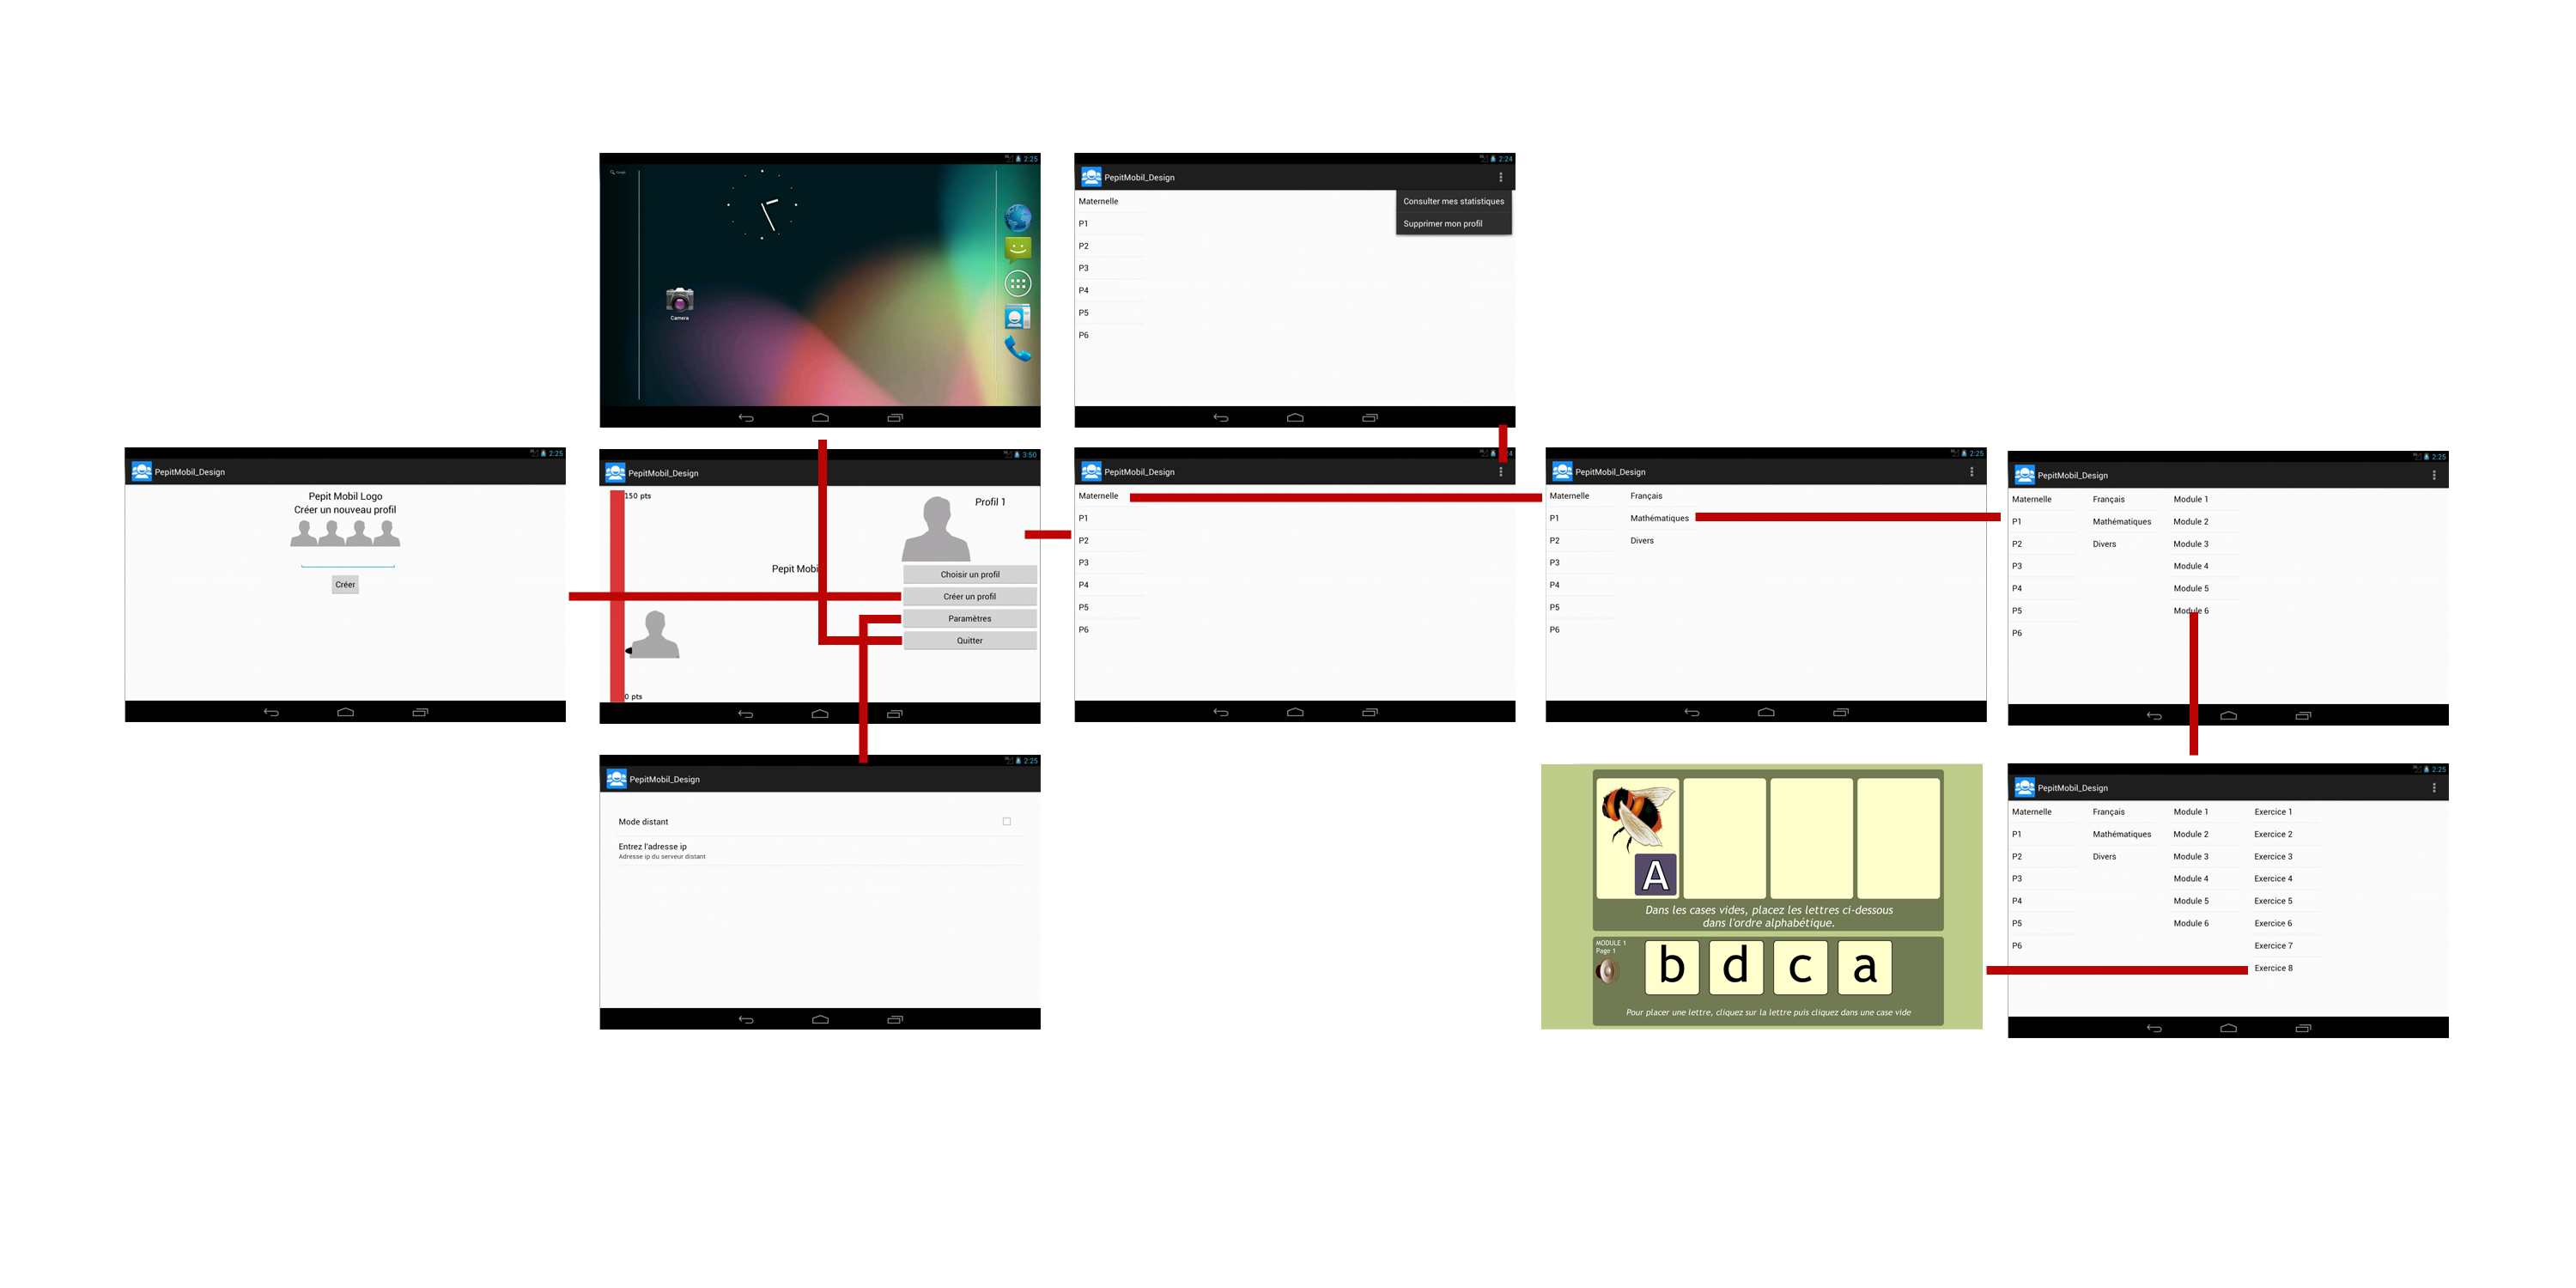
\includegraphics[width=20cm,angle=90]{images/pepit_wireframe}
\end{center}
\caption{Maquettes de l'application}
\label{Maquettes de l'application}
\end{figure}

toutes les maquettes se trouvent en annexe.

\subsection{Design}
\label{partie_design}
Le design de l'application est en cours de réalisation, pour celui-ci nous allons suivre le site déjà existant (pepit.be) ainsi que la charte graphique. Cette application est destinée aux enfants, il faut donc créer un design attractif.


La réalisation d'une icône est également indispensable pour une application mobile, celle-ci doit \^{e}tre assez claire et doit représenter le thème de l'application. Une première ébauche de celle-ci est disponible.


\begin{figure}[H]
\begin{center}

\includegraphics[width=8cm]{images/icone_2}
\end{center}
\caption{Icône Pepit Mobil}
\label{Icone Pepit Mobil}
\end{figure}
\subsection{Charte graphique}
\label{partie_charte_graphique}
\paragraph{}Elle va contenir l'ensemble des règles fondamentales d'utilisation des signes graphiques qui constituent l'identité graphique d'un projet.
\paragraph{}Dans ce document, nous avons défini les couleurs à utiliser pour le développement des exercices, pour garder une harmonie dans l'application. Egalement, nous allons y retrouver les maquettes du design avec les vues de l'application. En pièce jointe de cette charte, sera disponible les fichiers xml à utiliser dans le code pour le design des nouvelles activités de l'application. Pour l'instant le design n'est pas définitif, mais le sera prochainement.

%%% ************************************************** %
\section{3\ieme{} \sprint{}}
\label{sprint3}
\subsection{Herbegement du projet}
\label{hebergement_du_projet}
\paragraph{}Pour rappel, notre gestionnaire de développement est Github.
\paragraph{}Nous avons séparé le développement de l'application ma\^{i}tre et celui des plugins. Voici les différents comptes :
\begin{description}
\item[\href{https://github.com/pepit/PepitMobil}{Compte Pepit}] Celui-ci détient un dép\^{o}t, l'application ma\^{i}tre
\item[\href{https://github.com/pepit-team}{Organisation Pepit-Team}] Celui-ci détient les dép\^{o}ts des différents plugins
\end{description}

\subsection{Base de données}
\label{base_de_donnees}
Nous avons besoins de stocker des données au seins de notre application, pour les profils utilisateurs, les scores, la liste des exercices, ...


\subsubsection{SQLite 3}
C'est une base de données relationnelle écrite en langage C, qui est accessible en SQL. Cette base de données est directement intégrée dans les programmes, par rapport à MySQL et PostgreSQL qui sont des bases de données client-serveur. L'intégralité de la base de données (déclarations, tables, index et données) est stockée dans un fichier indépendant de la plateforme. Et surtout c'est cette base de données qui est préconisée sous Android.


Notre choix c'est porté sur SQLite 3, car celle-ci est directement utilisable dans Android.

\subsubsection{Dictionnaire de données}
\begin{tabbing}
\begin{tabular}{l l l l l}
	\hline
	Libellé de la propriété & Table & Nom du champ & Type & Taille \\
	\hline
	Numéro unique par niveau & levels & id & integer & \\	
	Nom du niveau & levels & name & varchar & 50 \\
	Alias du niveau & levels & label & varchar & 150 \\
	Description du niveau & levels & sub\_label & varchar & 150 \\
	Numéro unique par matière & subjects & id & integer & \\
	Nom de la matière & subjects & name & varchar & 50 \\
	Numéro du niveau lié à la matière & subjects & id\_level & integer	 & \\
	Numéro unique par thème & topics & id & integer & \\
	Nom du thème & topics & name & varchar & 50 \\
	Numéro de la matière lié à un thème & topics & id\_subject & 	integer & \\
	Nom du zip du plugin & topics & plugin\_name & varchar & 50 \\
	Description du thème & topics & label & varchar & 50 \\
	Numéro unique par profil & profils & id & integer & \\
	Nom du profil & profils & name & varchar & 50 \\
	Avatar du profil & profils & avatar & varchar & 10 \\
	Numéro unique par score & scores & id & integer & \\
	Numéro unique du plugin (topic) & scores & id\_plugin & integer & \\
	Numéro unique du profil & score & id\_profil & integer & \\
	Point par plugin (topic) & score & point & integer & \\
	Date du score & score & date & integer & \\
\end{tabular}
\end{tabbing}

\subsubsection{Modèle Conceptuel de Données}
\begin{figure}[H]
	\begin{center}
		\includegraphics[width=14cm]{\dossierimages mcd}
	\end{center}
	\caption{Maquettes de l'application}
	\label{Maquettes de l'application}
\end{figure}

\subsubsection{Model View Controler}
Nous avons mis en place un système se basant sur le système MVC, avec la création de modèles et de contr\^{o}lleurs. Ce qui simplifie le développement et la mise à jour.

\subsection{Navigation}
\label{navigation}
\subsubsection{Principes}
Le système de navigation est dynamique, lors d'un clique les informations de la colonne suivantes sont récupérer directement dans la base de données.

\subsubsection{En images}

\begin{figure}[H]
   	\begin{minipage}[c]{.46\linewidth}
		\includegraphics[width=7cm]{\dossierimages navigation_1}
		\caption{Navigation - Levels}
		\label{Navigation - Levels}
   	\end{minipage} \hfill
  	\begin{minipage}[c]{.46\linewidth}
      	\includegraphics[width=7cm]{\dossierimages navigation_2}
     	\caption{Navigation - Subjects}
		\label{Navigation - Subjects}
   	\end{minipage}
\end{figure}
\begin{figure}[H]
   	\begin{minipage}[c]{.46\linewidth}
		\includegraphics[width=7cm]{\dossierimages navigation_3}
		\caption{Navigation - Topics}
		\label{Navigation - Topics}
   	\end{minipage} \hfill
  	\begin{minipage}[c]{.46\linewidth}
      	
   	\end{minipage}
\end{figure}

\subsection{Importation des \plugin s}
\label{importation_plugin_sprint3}
\subsubsection{Les plugins}
Au niveau fichier, un plugin et un fichier \og{}zip\fg{} contenant le \jar{} (archive de classes java) de l'exercice ainsi que les ressources necessaire au bon fonctionnement de l'exercice placé dans 2 sous-dossier: \og{}drawable\fg{} et \og{}sounds\fg{}. Chaque plugin est donc constitué de cette façon.

Le nom du plugin est unique, c'est en fait une concaténation d'informations: le niveau de l'exercice, son thème ainsi que son nom. Par exemple \og{}m\_francais\_lelales\fg{} signifie que ce plugin correspond à l'exercice \og{}lelales\fg{}, qui est un exercice de français de niveau maternelle.

\subsubsection{Stockage des plugins}
\label{importation_plugin-stockage}
Tous les plugins seront mis à disposition dans un même dossier sur un serveur distant. Leur réferencement a lieu par le biai d'un fichier JSON. Ce fichier contient la liste trié (par niveau puis thème) de tous les plugins téléchargables.

Au niveau de l'application, les plugins téléchargés par l'utilisateur sont stockés localement sur l'appareil. Leur référencement ce fait par la base de données locale (voir la partie~\ref{base_de_donnees} pour plus de précision sur la base de données).

\subsubsection{Test accessibilité internet}
La tablette est capable de tester si l'accès internet est actif ou non sur la tablette à tout moment.

\subsubsection{Synchronisation des listes}
Une synchronisation de la liste des plugins disponibles sur le serveur distant se fait à chaque démarage de l'application si une connexion internet est disponible (actuellement sans demande de permition à l'utilisateur).
Cette synchronisation se fait de la manière suivante:
\begin{itemize}
    \item telechargement du fichier JSON
    \item lecture (avec paring) du fichier
    \item comparaison/synchronisation avec la \bdd{} locale:
    \begin{itemize}
        \item ajout de nouveaux plugins disponible
        \item actualisation du niveau de version disponible
        \item plugin devennu indisponible non géré (on considère que l'on ne retirera jamais d'exercice)
    \end{itemize}
\end{itemize}
%Téléchargement de la liste des plugins disponible: la liste des plugins disponibles est totalement géré (téléchargement et mise-à-jour), mais les niveaux et les thèmes sont encore insérés manuellement par l'application principale. 
%Cette mise-à-jour ce fait par le téléchargement du fichier JSON (voir partie~\ref{importation_plugin-stockage}), ce fichier est lu entièrement puis comparé avec la base de données locale afin de faire les ajouts/modifications nécessaires. 
Soulignons bien que cette procédure ne télécharge aucun \plugin{} et n'en mets aucun à jour. Elle actualise simplement la \bdd{} locale permettant ainsi de connaitre la liste totale de plugins disponible ainsi que leur numéro de version actuelle.

\subsubsection{Téléchargement}
\label{importation_plugin-telechargement}
Une fonction de téléchargement d'un plugin est disponible dans l'API mais n'est encore appelé à aucun endroit. Cette fonction télécharge par paquet l'archive du \plugin{} par rapport à son nom (unique) de \plugin{}.

\subsubsection{Amélioration prévus}
Il y a quatre principales améliorations à apporter à cette partie:
\begin{itemize}
    \item synchronisation totale de la liste des \plugin{}:
    \newline Comme dit précedament, seul les plugin sont mis-à-jour. La liste des niveaux et des thèmes et encore ajouter de manière manuelle dans l'applcation principale. La synchronisation doit donc toucher aussi ces deux niveaux (la \bdd{} locale sera complétement vide au premier lancement de l'application)
    \item téléchargement d'un \plugin{}:
    \newline La méthode le permettant est disponible mais non-utilisé.
    \item avertissement pour l'utilisateur:
    \newline Une demande de permission doit être faite à l'utilisateur pour toutes manipulations demandant un accès internet (en prévennant pour les coûts suplémentaires dû à la taille des plugins, etc)
    \item l'adresse du serveur distant:
    \newline Actuellement stocké en brut dans le code, elle devra être géré par rapport aux préférences
\end{itemize}


%%% ************************************************** %
\section{4\ieme{} \sprint{}}
\label{sprint4}
\subsection{Profils}
\label{profils}
\subsubsection{Généralités}
\paragraph{}Pepit mobil est une application multi-utilisateurs, un système d'utilisateur a été mis en place au sein de l'application. Le terme "profil" est utilisé pour un utilisateur, un profil pourra donc avoir ses propres exercices.

Un profil est défini avec :
\begin{itemize}
\item Un id
\item Un nom
\item Un avatar
\end{itemize}

\paragraph{}L'avatar sera sélectionné parmi une liste d'images libres de droit.

\subsubsection{Fonctionnalités}
Les fonctionnalités pour les profils sont les suivantes :
\begin{description}
\item[Création d'un profil] Sélection d'un avatar et d'un nom. Après validation, celui-ci devient le profil courant
\item[Suppression d'un profil] Ce qui entra\^{i}ne la suppression en cascade du score et des plugins téléchargés par ce profil
\item[Changement de profil] Chargement des différentes données du profil (avatar, nom, score, plugins)
\end{description}


\subsection{Amélioration de l'importation des \plugin s}
\label{importation_plugin_sprint4}
\subsubsection{Navigation et téléchargement d'un plugin}
Les \plugin s sont téléchargés lorsque l'utilisateur sélectionne un Topic (si le \plugin{} associé n'a jamais été téléchargé). Une demande lui ai faite pour savoir s'il veut vraiment télécharger et installer le plugin. 
Si oui, le plugin est téléchargé puis installé (installer veut aussi dire que l'on déclare le plugin disponible dans la \bdd{}).


%%%%%%%%%%%%%%%%%%%%%%%%%%%%%%%%%%%%%%%%%%%%%%%%%%%%%%%%%% Chap :
\chapter{Bilan et conclusion}
%% ************************************************** %
\section{Bilan}
\label{partie_bilan}
\textbf{Ce qui est fait :}
\begin{enumerate}
\item L'analyse des exercices
\item L'architecture de principale de l'application
\item Zoning des pages principales de l'application
\item Développement de l'architecture Android
\end{enumerate}

\textbf{Ce qui nous reste à faire :}
\begin{enumerate}
\item Application du style de l'application
\item Développement des exercices
\item Développement du système de plugins
\item Développement d'une API, pour la création de jeu
\end{enumerate}
%% ************************************************** %
\section{Avenir du projet}
\label{partie_avenir}
Le développement de l'application ne s'arrêtera pas avec notre projet, l'ambition du groupe est que celui-ci continue.


\subsection{Le projet}
Dans les mois futurs, l'application sera utilisé dans une école pour un test grandeur nature. 
Cela permettra d'avoir un grand nombre de retours avec les différents points de vues des utilisateurs ciblés (les enfants ainsi que les professeurs). 
Après celui-ci, nous aurons un retour concret sur les points qu'il nous reste à améliorer.


%L'équipe de projet est à la recherche de contributeurs au projet, pour l'évolution de l'application. Cette recherche pourra aboutir lors des projets informatique des Master de la promotion 2013/2014.

%Le projet est également à la recherche de développeur, pour réécrire les exercices présents sur le site web pepit.be gr\^{a}ce à l'API mise en place. Il est possible d'écrire des nouveaux exercices pour l'application.

L'équipe de projet est à la recherche de contributeurs. Les contributions pouvant être de différentes natures, principalement:
\begin{itemize}
    \item évolution de l'application maître
    \item ajout de contenus
    \item site vitrine
\end{itemize}

\subsubsection{\'{E}volution de l'appplication maître}
L'application maître à besoin encore d'un certain nombre d'ajout dont nous avons parlé précedement, par exemple:
\begin{itemize}
    \item amélioration du système d'importation d'un plugin
    \item lancement d'un plugin téléchargé (actuellement bogué)
\end{itemize}

\subsubsection{Ajout de contenus}
Concernant l'ajout de contenus, il s'agit principalement de la réecriture des exercices dans leur version \android{} (pour commencer car leur nombre est encore très limité).

\subsubsection{Site vitrine}
Le développement d'un site vitrine permettant d'ajouter/supprimer/consulter les exercices disponible sur le serveur est une évolution très interessante dont l'équipe avait parlé mais qui n'a pas encore était réalisé par manque de temps. Ce développement est donc à séparer des autres \og{}types\fg{} de contributions.

Cette vitrine pourrait permettre par exemple de:
\begin{itemize}
    \item gérer automatiquement le fichier JSON (ajout/suppression/modification d'un exercice)
    \item faciliter l'importation des exercices aux différents contributeurs
    \item faciliter la validation des exercices proposé (complétement manuel à l'heure actuelle)
    \item avoir un visuel du panel d'exercice disponible sans même avoir l'application
\end{itemize}


\subsection{L'équipe de développement}
Nous (Romain et Jonathan) voulons continuer à contribuer dans ce projet (en fonction de notre emploie du temps respectif). Cette motivation est dû à un int\^{e}ret pour les technologies mobiles tel que \android{} mais aussi à notre curiosité (nous souhaitons voir jusqu'où peut aller l'application \pepitMobil{}).

%% ************************************************** %
\section{Conclusion}
\label{partie_conclusion}
Dans un premier temps, nous souhaitons dire que participer à ce projet fût un immense plaisir. C'est un projet d'envergure selon nous étant donné l'affluence sur le site internet (200.000 visiteurs uniques). Il reste encore beaucoup de travail mais nous souhaitons que ce projet aille à son terme afin qu'il puisse aider à l'apprentissage d'un grand nombre d'enfants.

De plus, ce projet est une expérience d'importance dans notre cv, étant donné que nous sommes des acteurs de toutes les étapes du projet (analyse, conception, développement dans une nouvelle technologie, tests, ...).
Sans compter le fait qu'il est en parfaite adéquation avec notre master car c'est un projet libre utilisant des technologies abordées en cours.

Finalement, ce projet restera notre projet scolaire préféré. A tel point que nous souhaitons tous les deux le continuer en tant que contributeurs. Ce projet n'a pas été un jeu d'enfant, mais nous esperons de tout coeur qu'ils s'amuseront à apprendre avec.



%%%%%%%%%%%%%%%%%%%%%%%%%%%%%%%%%%%%%%%%%%%%%%%%%%%%%%%%%%%%%%%% ANNEXES
\appendix 
%%%%%%%%%%%%%%%%%%%%%%%%%%%%%%%%%%%%%%%%%%%%%%%%%%%%%%%%%% Chap :
\chapter{Références}
\begin{itemize}
\item[Pepit.be :] Site web pepit, portails de jeux éducatifs
\item[Zoning :] Maquette d'une application ou site internet, sans design mais juste l'emplacement des éléments
\item[API :] Une interface de programmation (Application Programming Interface ou API) est une interface fournie par un programme informatique. Elle permet l'interaction des programmes les uns avec les autres, de manière analogue à une interface homme-machine, qui rend possible l'interaction entre un homme et une machine.
\item[Activity :] Une activité est un composant d'une application qui fournit un écran avec lequel l'utilisateur peut interagir
\item[Google Play :] Boutique officiel d’application Android
\end{itemize}


%%%%%%%%%%%%%%%%%%%%%%%%%%%%%%%%%%%%%%%%%%%%%%%%%%%%%%%%%% Chap :
%\chapter{Scripts de réunions}
%\section*{1\iere{} réunion (29/10/2012)}
%\label{reunion1}
%% les includes sont incomplets, il faut préciser la plage de page qu'on importe
%\includepdf{\dossierpdf reunion1_29_10_2012_debut_du_projet}
%\section*{2\ieme{} réunion (26/11/2012)}
%\includepdf{\dossierpdf reunion2_26_11_2012}
%\section*{3\ieme{} réunion (17/12/2012)}
%\includepdf{\dossierpdf reunion3_17_12_2012}


%%%%%%%%%%%%%%%%%%%%%%%%%%%%%%%%%%%%%%%%%%%%%%%%%%%%%%%%%% Chap :
\chapter{Architecture}
\label{annexe_architecture}
\includepdf[page=1-3]{\dossierpdf scenario}


%%%%%%%%%%%%%%%%%%%%%%%%%%%%%%%%%%%%%%%%%%%%%%%%%%%%%%%%%% Chap :
\chapter{Maquettes}
\section*{Maquette - Page d'accueil}
\begin{figure}[H]
\begin{center}
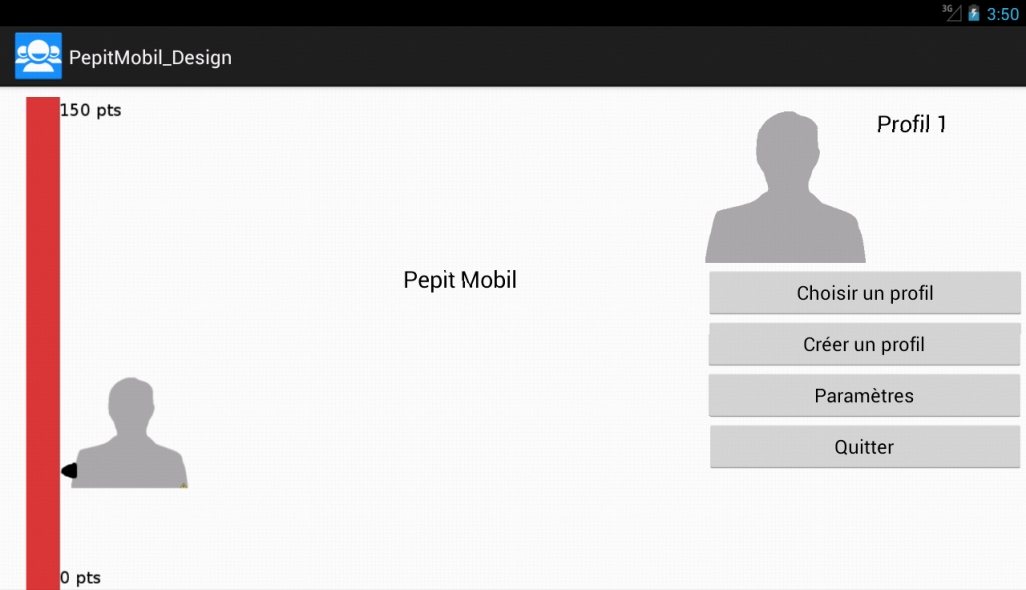
\includegraphics[width=15cm]{images/maquettes_homePage}
\end{center}
\caption{Pepit Mobil - Page d'accueil}
\label{Pepit Mobil - Page d'accueil}
\end{figure}

\section*{Maquette - Exercices}
\begin{figure}[H]
\begin{center}
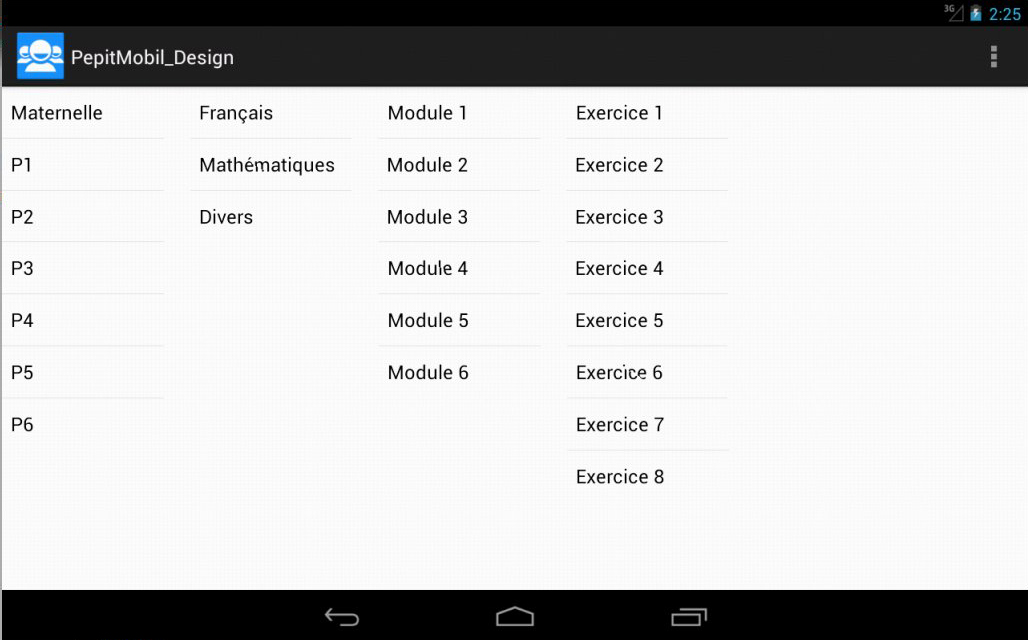
\includegraphics[width=15cm]{images/maquettes_exercices}
\end{center}
\caption{Pepit Mobil - Page exercices}
\label{Pepit Mobil - Page exercices}
\end{figure}

\section*{Maquette - Création de profil}
\begin{figure}[H]
\begin{center}
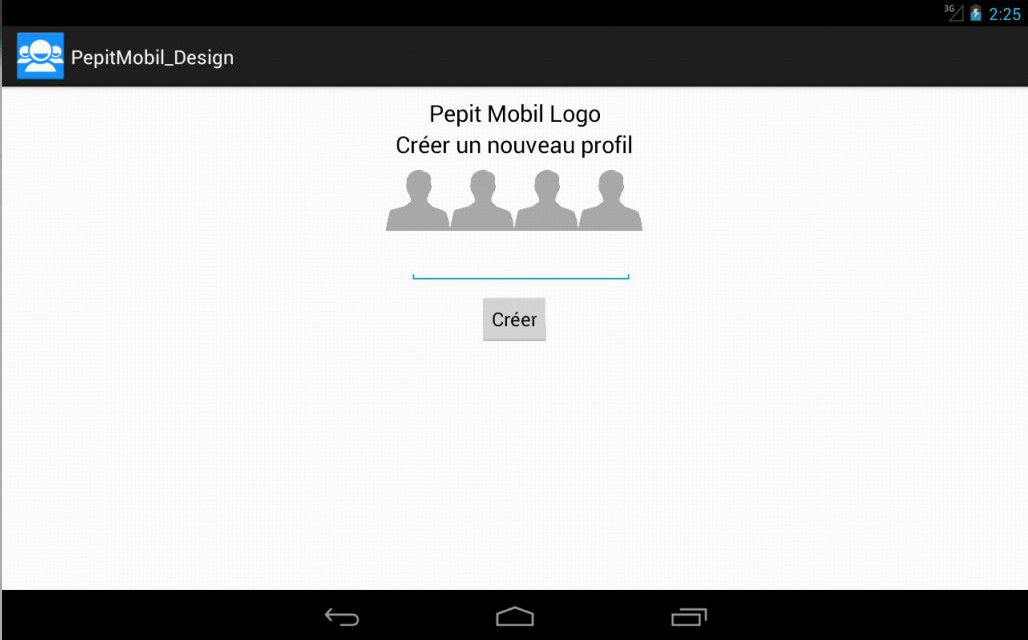
\includegraphics[width=15cm]{images/maquettes_creer_user}
\end{center}
\caption{Pepit Mobil - Page de création de profil}
\label{Pepit Mobil - Page de création de profil}
\end{figure}

\end{document}
